\chapter{Project description}
\textit{This chapter seeks to explain the design and implementation of the project along with the tests used for improving the system.}
\section{Architecture}
The architecture of the system explains the conceptual design blocks and interfaces. The architecture incorporates the requirements into a system and describes the overall structure and functionality of the system. 

\subsection{General system description}
The system consist of the CDU and a number of sensor nodes as seen on figure \ref{fig:systembdd}. The CDU is responsible for contacting the sensor nodes in order to collect and store the data that has been acquired by the sensor nodes. The sensor nodes sole responsibility is to acquire data.\\
The supply for the sensors nodes is taken from the custom power line communication bus. Communication signals between the CDU and sensor nodes are found on the bus as well. 
\begin{figure}[H]
	\centering
	\includegraphics[width=.9\textwidth]{billeder/11ProjectDescription/systembdd}
	\caption{System overview}
	\label{fig:systembdd}
\end{figure}
The general interface in the system is the bus. The sensor nodes are chain connected to the bus. The B+ connected is connected to the S+ of the first sensor in the chain. The next sensor in the chain is then connected with S+ to the S- of the first sensor. The last sensor in the chain is connected with S- to the B- on the CDU.\\
\subsection{System layers}
The CDU and the sensor nodes can be described as several layers with regards to communication as seen on figure \ref{fig:systemlayers}. Each layer handles different abstraction layers of the functionality and communication. 
\begin{figure}[H]
	\centering
	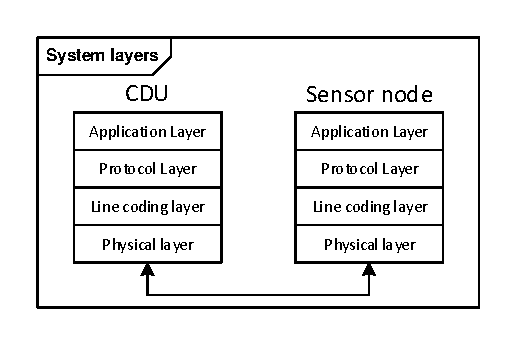
\includegraphics[width=.6\textwidth]{billeder/11ProjectDescription/System_Layers}
	\caption{System Layers}
	\label{fig:systemlayers}
\end{figure}
The model is inspired by the OSI model and each layers responsibility is as follows:
\begin{itemize}
	\item Application layer
	\subitem Found in the application layer is the entire application. Here all functionality is handled.
	\item Protocol layer
	\subitem Here the message comrised from the application layer is processed to comply with the protocol.
	\item Line coding layer
	\subitem The line coding layer converts the protocol message to comply with the line code specified to the bus.
	\item Physical layer
	\subitem The physical layer received the line coded stream of data and applies it to the bus be received by either the CDU or the Sensor node.
\end{itemize}
These layers help simplify the structure of the communication and the responsibility of each layer is very clear.
\subsection{CDU conceptual architecture}
Conceptual designs of the different parts of the system are made by taking the blocks from the system overview (figure \ref{fig:systembdd}) and creating internal block diagrams.\\
The internal block diagrams defines the internal structure of each block. These blocks should help make the functionality of each part possible and clearly define the boundaries within the part.\\
The CDU is comprised of six conceptual blocks as seen on figure \ref{CDU_IBD}. Each block has a unique responsibility. For instance the sensor power supply has the responsibility of powering the sensors. The sensor power supply block and sensor communication block makes up the physical layer with regards to figure \ref{fig:systemlayers} while the line coding and protocol layer is handled by the µ-Controller block. 
\begin{figure}[H]
	\centering
	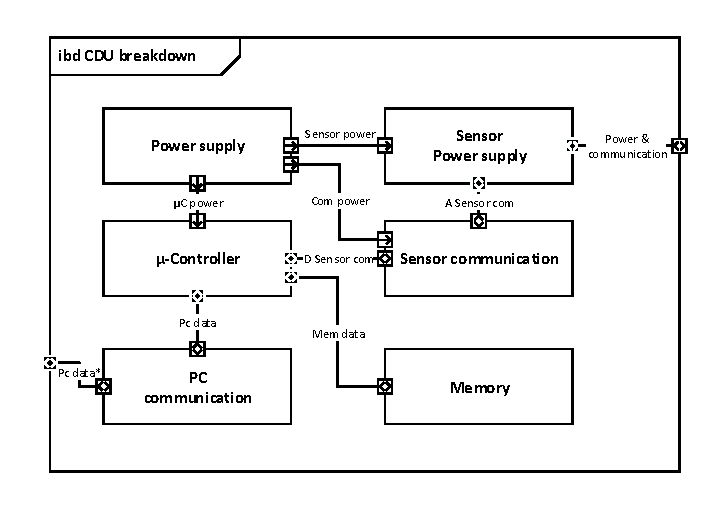
\includegraphics[width=.8\textwidth]{billeder/11ProjectDescription/CDU_IBD}
	\caption{Internal Block Diagram of the CDU}
	\label{CDU_IBD}
\end{figure}
\subsection{Sensor node conceptual architecture}
A sensor node can be divided into 4 conceptual blocks as seen on figure \ref{fig:SN_IBD}. The Power supply block and the Communication block make up the physical layer as described in the CDU. The line coding and protocol layer is handled by the Logic handler block.
\begin{figure}[H]
\centering
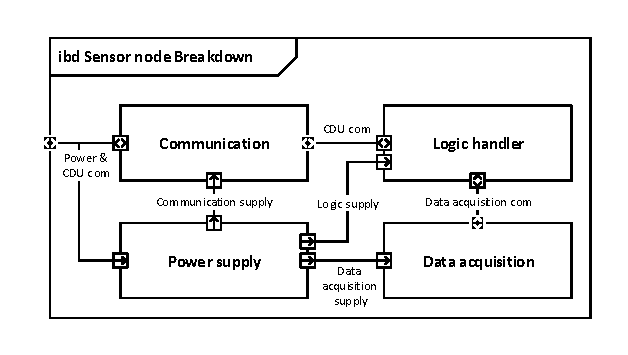
\includegraphics[width=.8\textwidth]{billeder/11ProjectDescription/Sensor_IBD}
\caption{Internal Block Diagram of the sensor node}
\label{fig:SN_IBD}
\end{figure}
\subsection{System communication}
The protocol is defined in the following section. The bus, named custom power line communication bus, has a header as seen below on table \ref{table:stdmsgtosensor}. The communication sequence is initiated by a start sequence. This sequence indicates the beginning of a transmission sequence. It is followed by an address and a function code. The address tells the sensor nodes which one is being contacted and the function code tells the sensor node how to react. The function codes is defined in a table found in the architecture document but and example could be the function code get data. When a sensor node receives this function code it responds with the data measured in the sensor and errors if any occured. The data length multiplier (DLM) defines how many bytes of data which is to be transmitted, and it can also be zero in which case no data is transmitted. This functionality is made to enable for variable message length so you don't waste time on sending dummy bytes etc. The data is then a multiple of the DLM in bytes. This could be the measured data from the sensor node to the CDU or it could be calibration data to the sensor node etc. Lastly the CRC is a standard cyclic redundancy check. The CRC is used to determine if the data was correctly received. If this is not the case the message is discarded. 
\begin{table}[hbpt]
	\centering
	\begin{tabular}{|l|l|l|l|l|l|}
		\hline
		Start Sequence & Address & Function Code & DLM & Data & CRC  \\ \hline
		1 nibble & 1 nibble	& 1 nibble & 1 nibble & n bytes & 1 byte\\
		\hline
	\end{tabular}
	\caption{Message format for writing and reading}
	\label{table:stdmsgtosensor}
\end{table}
Communication on the bus can be broken down to a series of steps. The CDU takes the initiative to write to a sensor node. It creates the message that will be sent and starts transmitting. The message is received on the sensor node and the sensor node starts processing the message. When it is finished processing it will respond according to the message. The response is received on the CDU where it will be processed. This transmission sequence can be seen on figure \ref{fig:sintrans}. The figure also shows the flow of information through the layers. 
\begin{figure}[H]
\centering
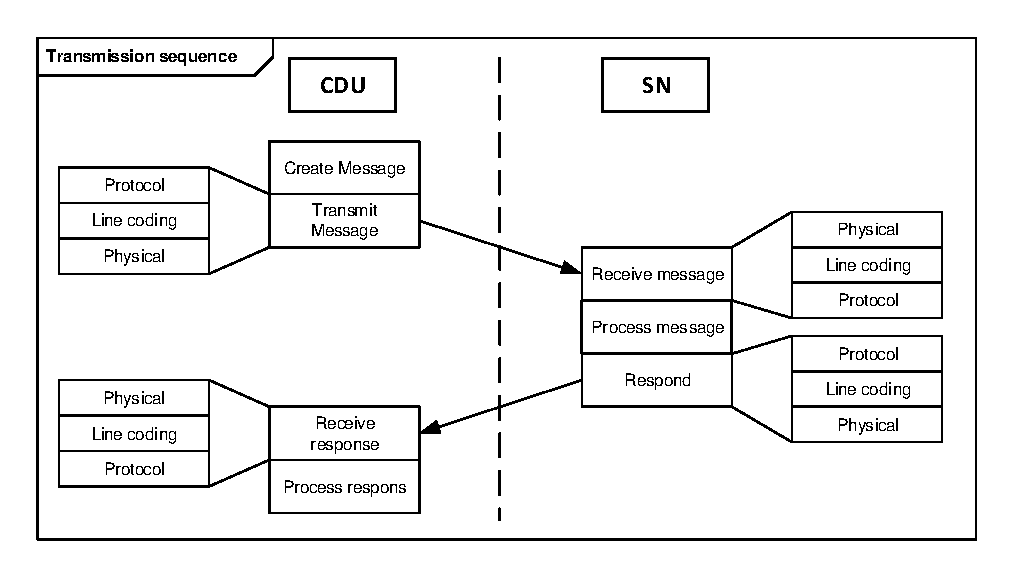
\includegraphics[width=.8\textwidth]{billeder/11ProjectDescription/singletransmission}
\caption{A single transmission}
\label{fig:sintrans}
\end{figure}

\section{Design and implementation}
The design and implementation of the system is a naturally continuation of the technology study made in this project. The key part was integrating the acquired knowledge from the study and applying it to design and implement the prototype system.\\
\subsection{Central data unit design}
The blocks from the architecture document were incorporated in order to create a detailed breakdown of the different parts of the system. The CDU block breakdown can be found in figure \ref{fig:detailedCDU}. The figure seeks to explain the block in a conceptual manner. The blocks and components inside the different design blocks explains the design choices. The block also contains the different external interfaces. \\
For the CDU there are three external interfaces with two pins each. These pins belong to the power supply block, the sensor power supply block and the pc communication block.\\
The brain of the CDU is the µ-Controller block. As seen on the figure, it contains a power line communication protocol block, a spi block and an uart block. The power line communication protocol block handles the protocol and line coding layer with respect to figure \ref{fig:systemlayers}.
\begin{figure}[H]
	\centering
	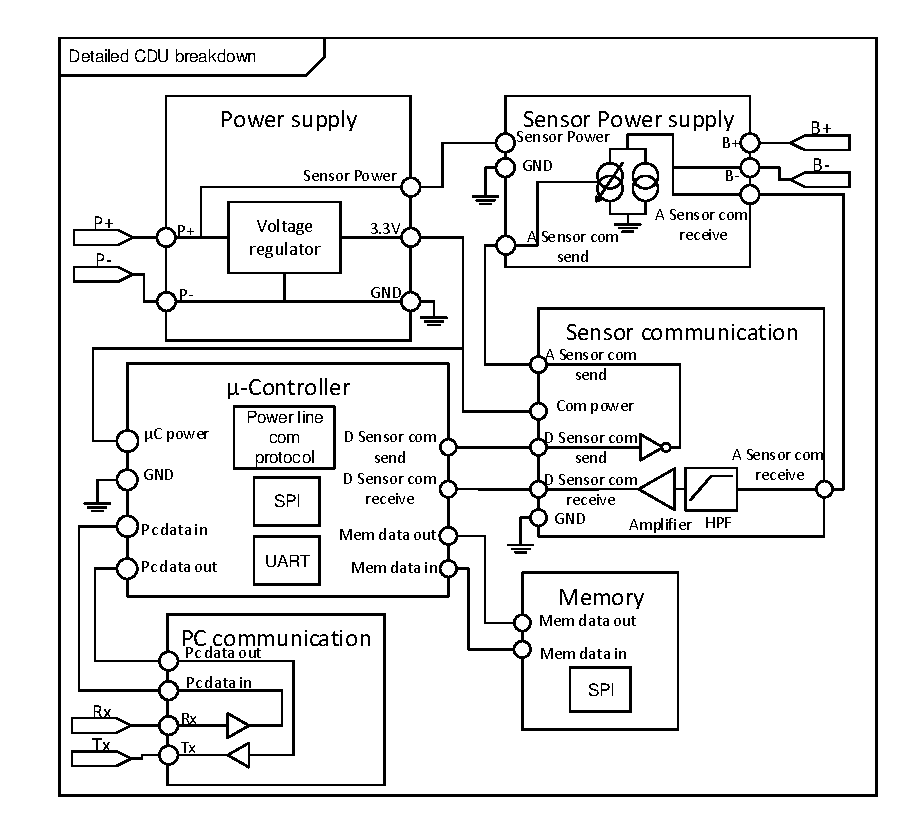
\includegraphics[width=0.8\textwidth]{billeder/11ProjectDescription/detailedCDU}
	\caption{Detailed CDU breakdown}
	\label{fig:detailedCDU}
\end{figure}
The design of the physical hardware layer was derived from the technology study of how a communication bus could be made. The central parts of the communication is carrying the communication and the conversion from digital levels to something that can be carried by the bus.\\ 
The during the technology study phase it became apparent that a current loop was the smartest way to communicate with- and power the sensor nodes. Two different current levels corresponds to logic 0(low) and 1(high). When responding, the sensor nodes use two different voltage levels.\\
The conversion from digital levels to analog current levels is handled by two block in the CDU: The Sensor power supply block (figure \ref{fig:CDUSPS}) and the Sensor communication block (figure \ref{fig:CDUSC}).
\begin{figure}[H]
	\begin{minipage}[b]{0.45\linewidth}
	\centering
	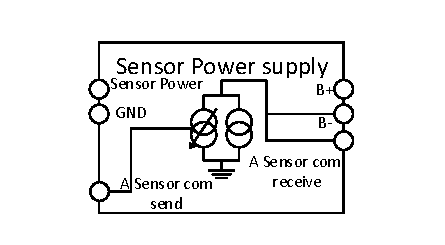
\includegraphics[scale=1]{billeder/11ProjectDescription/CDUSPS}
	\caption{Detailed CDU Sensor Power supply design.}
	\label{fig:CDUSPS}
	\end{minipage}
	\hspace{0.5cm}
	\begin{minipage}[b]{0.45\linewidth}
	\centering
	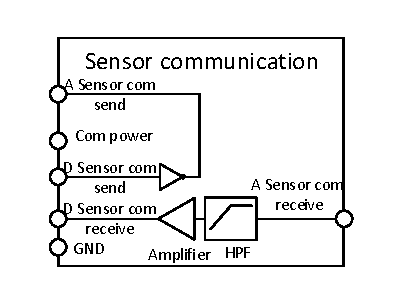
\includegraphics[scale=1]{billeder/11ProjectDescription/CDUSC}
	\caption{Detailed CDU Sensor communication design.}
	\label{fig:CDUSC}
	\end{minipage}
\end{figure}
The physical layer of the PC communication is handled by the PC communication block. The block contains conceptual level converters which are used to achieve the communication levels needed by the PC.\\
The memory block contains a spi block. This coincides with the µ-Controller block also containing a spi block as spi is used for communicating with the block. The memory is divided into sections containing the data specified in the requirement specification. This can be seen in memory allocation subsection of the software section of the design and implementation document.\\
The CDU is powered by the power supply block that contains a conceptual voltage regulator. Some blocks on in figure \ref{fig:detailedCDU} are implicitly supplied by the power supply.
\subsection{Sensor node design}
The sensor node breakdown can be found in figure \ref{fig:SN_detailed}. The figure contains both simple electronic components and conceptual blocks.\\
The brain of the sensor node is the logic handler. As seen on figure \ref{fig:SN_detailed} utilises the power line communication protocol and spi. The power line communication protocol bears great resemblance to the block of the same name in the CDU. The logic handler block communicates with the data acquisition block. The data acquisition block gathers data and holds it until it is requested by the logic handler. It is then stored on the logic handler until it is requested by the CDU.
\begin{figure}[H]
	\centering
	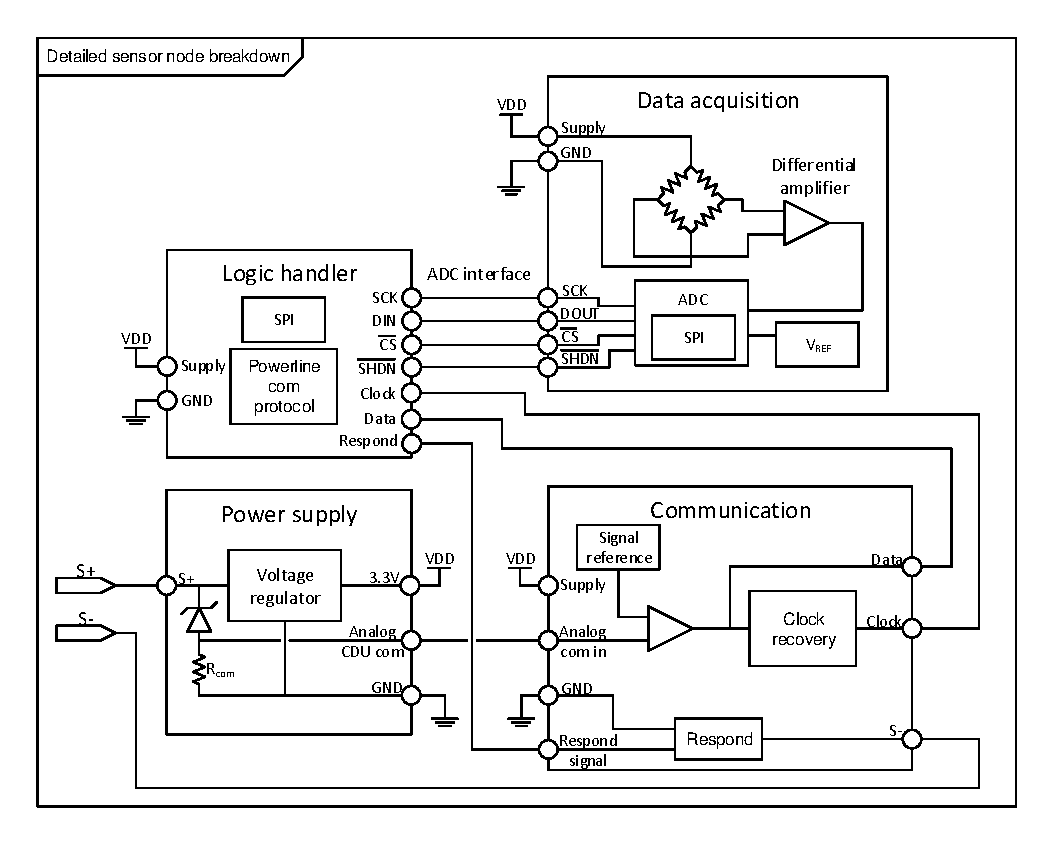
\includegraphics[width=0.8\textwidth]{billeder/11ProjectDescription/SN_detailed_design}
	\caption{Detailed sensor node breakdown}
	\label{fig:SN_detailed}
\end{figure}
When the CDU starts communicating on the custom power line communication bus, each sensor node will react to the difference in current levels. The current is converted to a voltage in the power supply block of the sensor node (figure \ref{fig:SN_PS_FIGURE}). The voltage levels are then converted to digital levels by the communication block of the sensor node(figure \ref{fig:SN_com_fig}).
\begin{figure}[H]
	\begin{minipage}[b]{0.45\linewidth}
	\centering
	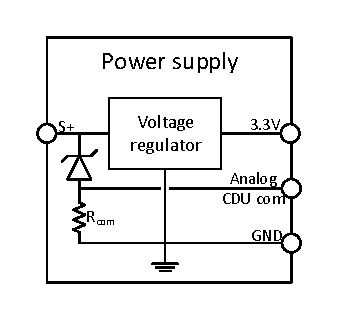
\includegraphics[width=0.8\textwidth]{billeder/11ProjectDescription/powersupply_detailed_sn}
	\caption{Sensor node power supply block}
	\label{fig:SN_PS_FIGURE}
	\end{minipage}
	\begin{minipage}[b]{0.45\linewidth}
	\centering
	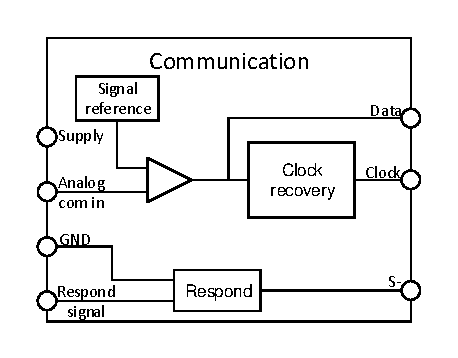
\includegraphics[width=1\textwidth]{billeder/11ProjectDescription/communication_sn}
	\caption{Sensor node communication block}
	\label{fig:SN_com_fig}
	\end{minipage}
\end{figure} 
Responding starts once the addressed sensor node has finished chewing through the message it has received. The digital level signal is converted to two different voltage levels by the communication block of the sensor node. The voltage levels on the bus is then directed from the sensor power supply of the CDU to the sensor communication block of CDU. The voltage levels will then be converted to digital logic levels and handled by the CDU.

\section{Prototype}
Realising the system meant taking the designs and making an initial prototype. The earliest versions of the prototypes were realised on breadboards. The first prototype provided a basis for testing the system and improving on the design. With the improvements to the design, the hardware was routed and put on PCBs. The tightly coupled hardware parts were put on the same PCB. The PCB blocks can be seen on figure \ref{fig:prototype}. The CDU prototype contains two circuit boards one made by the group and a development board. 
\begin{figure}[H]
	\centering
	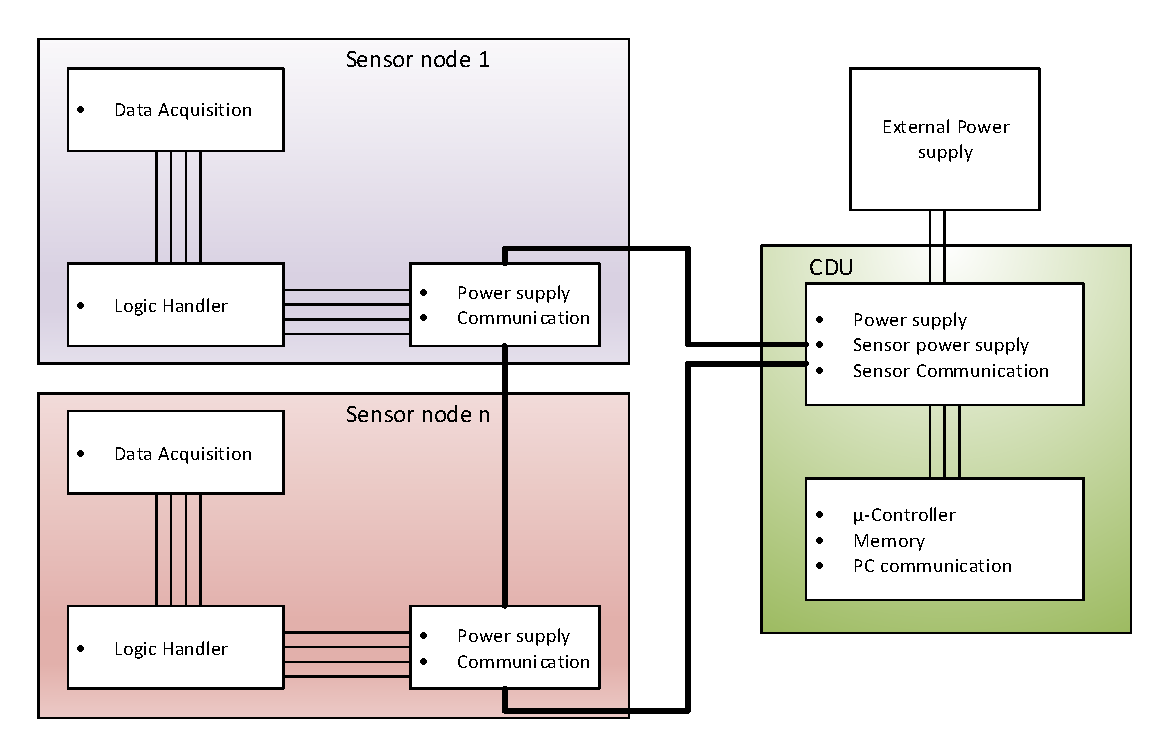
\includegraphics[width=0.8\textwidth]{billeder/11ProjectDescription/prototypesystem}
	\caption{Prototype system}
	\label{fig:prototype}
\end{figure}
The development board is an explorer 16 board. It contains a PIC24FJ chip, a memory chip and various level converters. The prototype CDU board contains a voltage regulator block, a constant current generator and an amplifier along with supporting circuitry.

The sensor nodes are comprised of three circuit boards. The data acquisition board, the logic handler board and the tighly coupled power supply and communication board. The logic handler board is an Altera DE2 board. The data acquisition board contains a measuring circuit and communication so that the logic handler can retrieve data. The power supply and communication board contains a CD4046 phase lock loop, a voltage regulator block, amplifiers and supporting circuitry. In the prototype there are two sensor nodes.

\subsection{Central data unit}
schematics printlayout sådan ngoet tænker jeg

\subsection{Sensor node}


\section{Tests}
\textit{The tests section seeks to explain the methods, reasons and procedures for testing in this project.}

The internal tests in this project is made up of unit tests and integration tests. The unit tests seek to tests the functionality of each device while the integration tests are designed to tests the communication in between devices.

The unit tests were made such that there were as few variable circumstances as possible. This means possible errors will most certainly stem from the unit under test (uut). This principle of testing was also applied when unit testing.

The tests made in this project are by no means exhaustive. The tests made are suppose to provide a baseline for improving the system or otherwise prove a basic concept. As the outcome of this project is a technology and not an actual product there is no accept-test.

The full extent of tests are:\\
\begin{table}[H]
	\centering
    \begin{tabular}{|p{6.5cm}|p{7.5cm}|}
    \hline
    Integration test case                       & Goal: \\ \hline
    1: Sensor getinfo request                   & To test the communication from CDU to Sensor node\\ \hline
    2: Sensor getdata request                   & ---||--- \\ \hline
    3: Sensor respond to getinfo                & To test the communication from Sensor node to CDU\\ \hline
    4: Sensor respond to getdata                & ---||--- \\ \hline
    5: Full transmission                        & To test the full communication scheme     \\ \hline
    6: Full transmission, unknown function code & To test the error responding scheme     \\ \hline 
    7: PC sends getdata request to CDU          & To test the communication with the PC     \\ \hline
    8: PC sends unknown request to CDU          & To test the error in communication with the pc\\ \hline
    \end{tabular}
    \caption{Integration test cases}
    \label{tab:intetestcas}
\end{table}
\begin{table}[H]
	\centering
    \begin{tabular}{|p{6.5cm}|p{7.5cm}|}
    \hline
    Reliability test case                             & Goal: \\ \hline
    1: Timed transmissions and errors                 & To test the reliability of the bus \\ \hline
    \end{tabular}
    \caption{Reliability test cases}
    \label{tab:reliability}
\end{table}
\begin{table}[H]
	\centering
    \begin{tabular}{|p{6.5cm}|p{7.5cm}|}
    \hline
    CDU unit test case                             & Goal: \\ \hline
    1: 3.3 volt power supply                       & To test the power supply block\\ \hline
    2: Communication to bus                        & To test the sensor communication block     \\ \hline
    3: Voltage reference in receiver circuit       & ---||---     \\ \hline
    4: Communication from bus                      & ---||---     \\ \hline
    5: Test of function IntegerToBinary            & Software test of function     \\ \hline
    6: Test of function PatMessage                 & ---||---     \\ \hline
    7: Test of function ToManchester               & ---||---     \\ \hline
    8: Test of function InitSensorArray            & ---||---     \\ \hline
    9: Test of function CDUSend                    & ---||---     \\ \hline
    10: Test of function CDUReceive                & ---||---     \\ \hline
    11: Test of function CDUReceive error handling & ---||---     \\ \hline
    \end{tabular}
    \caption{CDU unit test cases}
    \label{tab:cduutc}
\end{table}
\begin{table}[H]
	\centering
    \begin{tabular}{|p{5.5cm}|p{8.5cm}|}
    \hline
    Sensor node unit test case                  & Goal: \\ \hline
    1: 3.3 volt power supply                    & To test the power supply block\\ \hline
    2: Data recovery circuit                 	& To test the data recovery of the communication block     \\ \hline
    3: Phase lock circuit               		& To test the phase lock of the communication block     \\ \hline
    4: Respond circuit               			& To test the respond circuit of the communication block     \\ \hline
    5: CDU communication                        & To test line coding and protocol layers of the logic handler block\\ \hline
    6: ADC interfacing 							& To test the interface of the ADC     \\ \hline 
    \end{tabular}
    \caption{Sensor node unit test cases}
    \label{tab:SNUT}
\end{table}
The content of a test can be explained on the basis of integration test case 1 which can be found in the Internal tests document in the appendix. Each test case contains the purpose of the tests, which tests equipment is used in the test, the procedure, the expected result and the actual result.\\ 
The purpose explains what is being tested. The test equipment used includes stubs of the units that are being tested. This could be a sensor stub needed for testing the CDU or a full sensor node tests stub used for testing communication. The procedure seeks to explain how to do the tests in a way such that a technician can perform the test without prior knowledge to the system. The expected result provides a range or a basis on which the actual result can be evaluated.\\